\documentclass{article}
\usepackage[letterpaper]{geometry}
\geometry{verbose,tmargin=1in,bmargin=1in,lmargin=1in,rmargin=1in}

\usepackage[utf8]{inputenc}
\usepackage{amsmath}
\usepackage{float}
\usepackage{listings}
\usepackage{graphicx}
\usepackage{enumitem}

\title{CIS 419/519: Homework 3}
\author{\{Yupeng Li\}}
\date{02.20.2020}

\begin{document}
    \maketitle
    Although the solutions are entirely my own, I consulted with the following people and sources while working on this homework:
    
    \section{Logistic Regression}
    	\subsection{Implementation}
	This section is done in the python file with both L1 regularization and L2 regularization implementations.
	
	\subsection{Testing Your Implementation}
	In this section, the implementation of the logistic regression is tested dataframe and yields a similar result in the assignment PDF. The results are in the figure below:
		\begin{figure}[H]
			\caption{Graph under L2 norm and $\lambda$ = 1E-9}
			\centering
			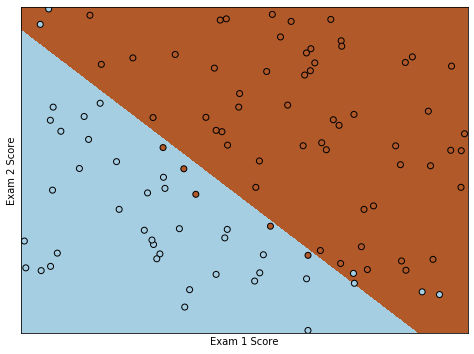
\includegraphics[width=8cm]{LinearL2norm.png}
		\end{figure}

	\subsection{Analysis}
	In this part, we would compare the results for logistic regression based on different $\lambda$ and under situations of 1 norm and 2 norm:
		\begin{figure}[H]
			\caption{Graph under L2 norm and $\lambda$ = 10}
			\centering
			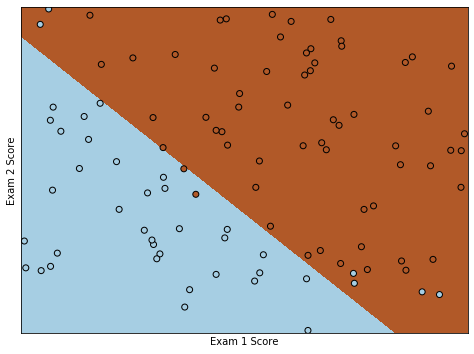
\includegraphics[width=8cm]{LinearL2norm10.png}
		\end{figure}
		\begin{figure}[H]
			\caption{Graph under L1 norm and $\lambda$ = 1E-9}
			\centering
			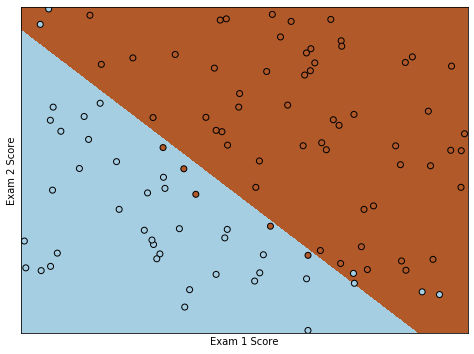
\includegraphics[width=8cm]{LinearL1norm0.png}
		\end{figure}
			\begin{figure}[H]
			\caption{Graph under L2 norm and $\lambda$ = 10}
			\centering
			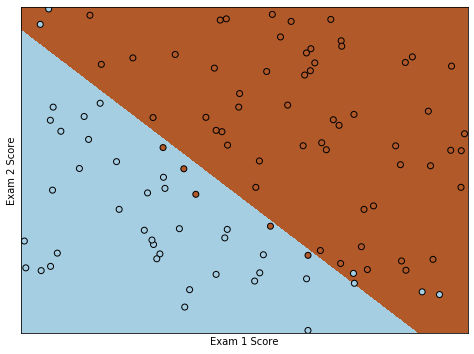
\includegraphics[width=8cm]{LinearL1norm10.png}
		\end{figure}
		\\
		
	We can see from the figures that, with almost 0 regularization constant, both L1 norm result and L2 result are exhibiting similar pattern with no significant difference. While when the regularization constant is raised to 10, the L2 regularization pushes the decision boundary slightly forward towards negative while the results of L1 regularization stays almost the same.
	
	\subsection{Learning a non-linear decision surface}
	This part is in the submitted .py file
	The following graph demonstrates how the non-linear decision surface works with almost 0 L2 regularization
	\begin{figure}[H]
			\caption{Graph under L2 norm and $\lambda$ = 1E-9}
			\centering
			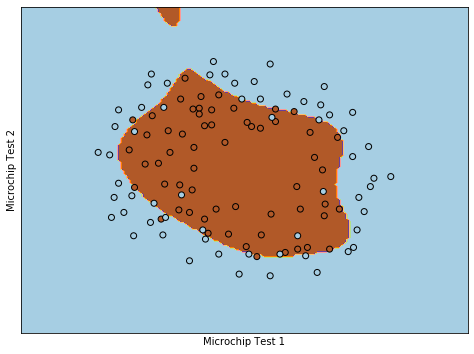
\includegraphics[width=8cm]{NonlinearL2norm0.png}
		\end{figure}
	\section{Comparing Algorithms}
		\subsection{Logistic Regression Adagrad}
		The logistic Adagrad has been implemented and submitted through gradescope in the .py file
		\subsection{Comparing Algorithms}
		According to \{https://www.kaggle.com/uciml/pima-indians-diabetes-database\}
		\\There 758 samples in total in this dataset with 8 attributes with no missing data\\
		
		Each column in hw3.diabetes dataset stand for the items as following :
		\begin{itemize}
			\item Pregnancies Number of times pregnant
			\item GlucosePlasma glucose concentration a 2 hours in an oral glucose tolerance test
			\item BloodPressure Diastolic blood pressure (mm Hg)
			\item SkinThickness Triceps skin fold thickness (mm)
			\item Insulin2-Hour serum insulin (mu U/ml)
			\item BMIBody mass index weight in $kg/(height in m)^2$
			\item Diabetes PedigreeFunctionDiabetes pedigree function
			\item Age Age (years)
			
		\end{itemize}

		The last column of the data frame stand for the outcome in 'tested\_negative' and 'tested\_postive', preprocessing has been done for the last column to convert the results into booleans of 1s and 0s.\\
		\\
		Under CrossValidation with 5 folds and 5 trials, different algorithms give different results
		\begin{itemize}
		\item L1 Logistic Regression with $\lambda$ = 1, CVScore = 0.7648
		\item L2 Logistic Regression with $\lambda$ = 1, CVScore = 0.7669
		\item L1 Logistic Adagrad Regression with $\lambda$ = 1, CVScore = 0.651
		\item L2 Logistic Adagrad Regression with $\lambda$ = 1, CVScore = 0.662
		\end{itemize}\\
		\\
		According to the \{\https://archive.ics.uci.edu/ml/datasets/Breast+Cancer+Wisconsin+(Diagnostic)}
		
		

The columns here stand for:\\
a) radius (mean of distances from center to points on the perimeter)\\
b) texture (standard deviation of gray-scale values) \\
c) perimeter \\
d) area \\
e) smoothness (local variation in radius lengths) \\
f) compactness ($\frac{perimeter^2}{area - 1.0}$) \\
g) concavity (severity of concave portions of the contour)\\ 
h) concave points (number of concave portions of the contour)\\ 
i) symmetry \\
j) fractal dimension ("coastline approximation" - 1)\\

		\\There 569 samples in total in this dataset with 30 attributes with no missing data\\

		Under CrossValidation with 5 folds and 5 trials, different algorithms give different results
		\begin{itemize}
		\item L1 Logistic Regression with $\lambda$ = 1, CVScore = 0.9729
		\item L2 Logistic Regression with $\lambda$ = 1, CVScore = 0.97714
		\item L1 Logistic Adagrad Regression with $\lambda$ = 0.01, CVScore = 0.9743
		\item L1 Logistic Adagrad Regression with $\lambda$ = 1, CVScore = 0.62737
		\item L2 Logistic Adagrad Regression with $\lambda$ = 1, CVScore = 0.9307
		\end{itemize}\\

\\According to the \{https://archive.ics.uci.edu/ml/datasets/Diabetic+Retinopathy+Debrecen+Data+Set\}
\\There is no missing data in this data set, there are 1151 instances in this sample with 19 aspects.\\
The attributes are \\\\
0) The binary result of quality assessment. 0 = bad quality 1 = sufficient quality.\\ 
1) The binary result of pre-screening, where 1 indicates severe retinal abnormality and 0 its lack. \\
2-7) The results of MA detection. Each feature value stand for the 
number of MAs found at the confidence levels alpha = 0.5, . . . , 1, respectively. \\
8-15) contain the same information as 2-7) for exudates. However, 
as exudates are represented by a set of points rather than the number of 
pixels constructing the lesions, these features are normalized by dividing the 
number of lesions with the diameter of the ROI to compensate different image 
sizes.\\
16) The euclidean distance of the center of 
the macula and the center of the optic disc to provide important information 
regarding the patient’s condition. This feature 
is also normalized with the diameter of the ROI. \\
17) The diameter of the optic disc. \\
18) The binary result of the AM/FM-based classification. \\
19) Class label. 1 = contains signs of DR (Accumulative label for the Messidor classes 1, 2, 3), 0 = no signs of DR.\\

		Under CrossValidation with 5 folds and 5 trials, different algorithms give different results
		\begin{itemize}
		\item L1 Logistic Regression with $\lambda$ = 1, CVScore = 0.6503
		\item L2 Logistic Regression with $\lambda$ = 1, CVScore = 0.5930
		\item L1 Logistic Adagrad Regression with $\lambda$ = 1, CVScore = 0.5308
		\item L2 Logistic Adagrad Regression with $\lambda$ = 1, CVScore = 0.6036
		\end{itemize}\\


		\subsection{Understanding Regularization and Adagrad}
		\begin{figure}[H]
			\caption{Logreg Graph under L2 norm and $\lambda$ = 1, $\alpha$ = 1}
			\centering
			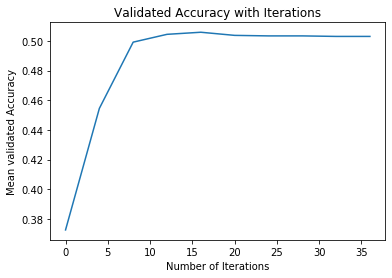
\includegraphics[width=8cm]{LogNorm2.png}
		\end{figure}

		\begin{figure}[H]
			\caption{Logreg Graph under L1 norm and $\lambda$ = 1, $\alpha$ = 1}
			\centering
			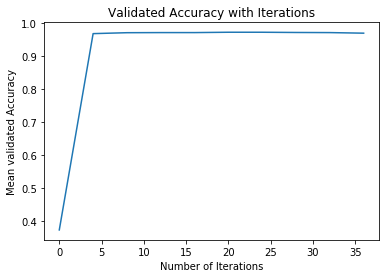
\includegraphics[width=8cm]{LogNorm1.png}
		\end{figure}
		
		\begin{figure}[H]
			\caption{Adagrad Graph under L2 norm and $\lambda$ = 1, $\alpha$ = 1}
			\centering
			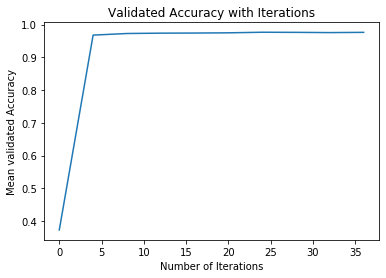
\includegraphics[width=8cm]{AdaNorm2.png}
		\end{figure}
		
		
		\begin{figure}[H]
			\caption{Adagrad Graph under L1 norm and $\lambda$ = 0.01, $\alpha$ = 1}
			\centering
			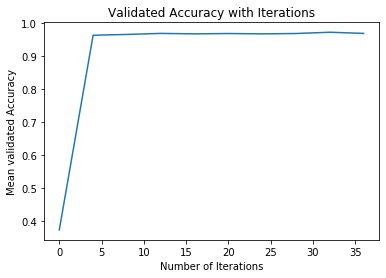
\includegraphics[width=8cm]{AdaNorm1.png}
		\end{figure}
	

From the results above, we can conclude that if starting with a poorly chosen fixed learning rate $\alpha$, the converging will become very slow with normal logistic regression. However, if we change the regularization factor from 2 norm to 1 norm, it will actually converge faster. Meanwhile, changing from fixed learning rate to adaptive regression will help improve the learning efficiency. From the graphs, it is clear that the one adapting Adagrad 2 L2 norm converges way faster than its counterpart in Logistic regression. Thus we can conclude that, adagrad is good at fixing a poorly chosen $\alpha$ and helps the system converge at a much higher speed. It is not necessarily always faster than logistic regression, but it does help to prevent falling into the infinitely approaching loop.


        
\end{document}